%%%%%%%%%%%%%%%%%%%%%%%%%%%%%%%%%%%%%%%%%%%%%%%%%%%%%%%%%%%%%%%%%%%%%%%%%%%%%%%%
%2345678901234567890123456789012345678901234567890123456789012345678901234567890
%        1         2         3         4         5         6         7         8

\documentclass[letterpaper, 10 pt, conference]{ieeeconf}  % Comment this line out
                                                          % if you need a4paper
%\documentclass[a4paper, 10pt, conference]{ieeeconf}      % Use this line for a4
                                                          % paper

\IEEEoverridecommandlockouts                              % This command is only
                                                          % needed if you want to
                                                          % use the \thanks command
\overrideIEEEmargins
\usepackage{graphicx}
% See the \addtolength command later in the file to balance the column lengths
% on the last page of the document



% The following packages can be found on http:\\www.ctan.org
%\usepackage{graphics} % for pdf, bitmapped graphics files
%\usepackage{epsfig} % for postscript graphics files
%\usepackage{mathptmx} % assumes new font selection scheme installed
%\usepackage{times} % assumes new font selection scheme installed
%\usepackage{amsmath} % assumes amsmath package installed
%\usepackage{amssymb}  % assumes amsmath package installed

\title{\LARGE \bf
Spatial-Temporal Deep Neural Networks for Land Use Classification of LandSat Images
}

%\author{ \parbox{3 in}{\centering Huibert Kwakernaak*
%         \thanks{*Use the $\backslash$thanks command to put information here}\\
%         Faculty of Electrical Engineering, Mathematics and Computer Science\\
%         University of Twente\\
%         7500 AE Enschede, The Netherlands\\
%         {\tt\small h.kwakernaak@autsubmit.com}}
%         \hspace*{ 0.5 in}
%         \parbox{3 in}{ \centering Pradeep Misra**
%         \thanks{**The footnote marks may be inserted manually}\\
%        Department of Electrical Engineering \\
%         Wright State University\\
%         Dayton, OH 45435, USA\\
%         {\tt\small pmisra@cs.wright.edu}}
%}

\author{Cameron Farzaneh$^{1}$, Atharva Sharma, PhD$^{1}$, Xiuwen Liu, PhD$^{1}$, Xiaojun Yang, PhD$^{2}$, Di Shi, PhD$^{3}$% <-this % stops a space
\thanks{$^{1}$Department of Computer Science, Florida State University, Tallahassee, FL 32306-4530, United States}%
\thanks{$^{2}$Department of Geography, Florida State University, Tallahassee, FL 32306-2190, United States}%
\thanks{$^{3}$Department of Geography and Atmospheric Science, University of Kansas, Lawrence, KS 66045-7316, United States}%
}

\begin{document}



\maketitle
\thispagestyle{empty}
\pagestyle{empty}


%%%%%%%%%%%%%%%%%%%%%%%%%%%%%%%%%%%%%%%%%%%%%%%%%%%%%%%%%%%%%%%%%%%%%%%%%%%%%%%%
\begin{abstract}

To maintain global environment sustainability, an availability of accurate land cover information over large areas is essential. The means in which this data can be obtained is through digital class-action using medium-resolution remote sensing information. This would provide an effective method of generating the land cover information that is required. However, the existence of low accurate pixel-based classification methods for medium-resolution data is a limitation. Convolutional Neural networks (CNNs) have been achieving remarkable improvements in object recognition applications and classification, however, they rely on fine image structures. Due to the limitation of data being at medium resolution, standard CNNs cannot be applied directly due to lack of fine structures in the dataset. In this research, a new patch-based CNN tailored for medium-resolution remote sensing data that was initially proposed by Dr. Sharma is implemented. This CNN considers the spatial relation of a pixel to its neighborhood by computing patch-based samples from multidimensional top-of-atmosphere reflectance data. Initially, patches of pixel size 5 $\times$ 5 $\times$ 8 are extracted and analyzed. In addition, different patch sizes are extracted and analyzed in order to explore the significance on the model. It appears that validation accuracy improves as patch size increases. 3 $\times$ 3 $\times$ 8 achieves 79\% accuracy, 5 $\times$ 5 $\times$ 8 achieves 89\% accuracy, 7 $\times$ 7 $\times$ 8 achieves 93\% accuracy, 9 $\times$ 9 $\times$ 8 achieves 96\% accuracy, and 11 $\times$ 11 $\times$ 8 achieves 98\% accuracy. To understand why the accuracy increases, we look into the patches itself. With using a test site from the Florida Everglades with an area of 771 square kilometers, this patch-based CNN outperform pixel-based neural network, pixel-based CNN and patch-based neural network by 24.36\%, 24.23\% and 11.52\%, respectively, in overall classification test accuracy. By using this proposed patch-based CNN along with the vast availability of medium-resolution remote sensing data, more accurate land cover datasets can be built over large areas.

\end{abstract}


%%%%%%%%%%%%%%%%%%%%%%%%%%%%%%%%%%%%%%%%%%%%%%%%%%%%%%%%%%%%%%%%%%%%%%%%%%%%%%%%
\section{INTRODUCTION}

Land cover, the physical material that covers the surface of our planet, is an important form of data that is essential to global environment sustainability. Its use has many applications in the fields of environmental science, land management and geography. Because of the importance of land cover information, there have been many efforts to generate large amounts of land cover datasets. But simply having large amounts of the data is not enough; the data must be processed and observed. This is generally achieved through ground surveys and/or remote sensing. Ground surveys, although very accurate, are limited by logistic constraints making it not a feasible option to cover most of our large planet. Remote sensing, on the other hand, is the favored method because it takes advantage of cameras and sensors that are installed on satellites and observe large areas of land surface of Earth over time. This allows an efficient and affordable method to map land cover patters. Luckily, there is an abundance of publicly available and free of charge remote sensing data at medium-resolution such as Landsat imagery (USGS, 2016a). This data includes aerial photographs, satellite imagery, thermal imagery, hyper-spectral imagery, radar and lidar datasets; which vary in spatial, spectral, radiometric and temporal resolutions. Using the vast amount of data available, both visual interpretation and computer based digital classification can be used to extract information about land cover. Generally, digital pattern classification is the preferred method of mapping land cover in large areas over visual interpretation. Now that there is remote sensing data with improved spectral, spatial and temporal resolutions available to the community, the real problem is to effectively and accurately use this data for image classification for land cover use.

The remote sensing community has many advances with conventional methods such as maximum likelihood classifier (MLC) (Strahler, 1980) and clustering (Huang, 2002). More recently, it has now moved towards more advanced techniques such as decision trees (Xu, Watanachaturaporn, Varshney, \& Arora, 2005), random forests (RF) (Pal, 2005), neural networks (NN) (Kavzoglu \& Mather, 2003; Mas \& Flores, 2008), support vector machines (SVM) (Gidudu, Hulley, \& Marwala, 2007; Mountrakis, Im, \& Ogole, 2011; Pal \& Mather, 2005) and convolutional neural networks (CNN) (Castelluccio, Poggi, Sansone, \& Verdoliva, 2015; Romero, Gatta, \& Camps- Valls, 2016) to preform classification on the remote sensing data. Deep neural networks have recently showed to achieve significant empirical improvements in various fields such as computer vision and natural language processing. An example of this can be seen with the ImageNet competition and the fact that CNNs have surpassed human performance on the ImageNet dataset. This dataset consists of 1000 classes and contains 1.2 million training images with 50,000 validation and 100,000 test images. Utilizing the same techniques that CNNs can achieve can have a large impact on remote sensing classification if used correctly. For remote sensing classification, CNNs are not a new approach, however. Although there has already been research done using CNNs on remote sensing classification, smaller datasets with high-resolution images were being used. This is because classification of high-resolution images is similar to object recognition in computer vision. As a result, these CNNs have been shown to work well on high-resolution remote sensing images. While this is a great achievement, the architecture is limited in that it depends on high-resolution images. It is currently difficult to obtain high-resolution images that not only cover all areas of our planet, but also span a very large area. On the other hand, there is plenty of medium-resolution remote sensing data available from the Landsat satellite that is public and free. The satellite also provides the longest continuous observations of Earth’s surface from space. The Landsat system provides copious amounts of highly calibrated, multi-spectral data of global coverage. For there to exist an accurate form of classifying medium resolution imagery would be a large advantage as it combines the power of CNNs along with the abundance of ready-to-use medium-resolution images. \\ \indent Although the problem of obtaining a large enough dataset has been solved curtesy of the Landsat program, we cannot simply construct any convolutional neural network and expect good results. This is because current deep neural networks using pixel-based approach, when applied to medium-resolution data, have not been able to achieve good accuracy. Most previous techniques to classify medium-resolution remote sensing are all pixel-based. An example of this can be seen with MLC, decision trees, RF and SVM all obtaining an overall accuracy of 64.9\% for producing a 30 m resolution global land-cover dataset. While these results can still be applied in certain fields, it may not be enough to support different applications that require the land-cover information to be more accurate. The main goal of this research is to implement a deep neural network for land cover classification using medium-resolution satellite imagery, while also experimenting with various sized inputs in hopes to find an optimal architecture that can achieve the largest accuracy on medium-resolution data. Using the fact that a pixel is spatially related to its neighborhood, a six-layer deep convolutional neural network that has initially been proposed by Dr. Sharma and has achieved better accuracy can be applied to medium-resolution data such as the Landsat dataset. Because the dataset consists of 30 m spatial resolution of non-thermal bands, typical CNN architectures without any modification will not be effective because of the lack of quality in the image. This is due to the fact that CNN architectures for object recognition normally depend on features such as shape, texture and other fine structures in order to detect small objects like houses. In medium-resolution datasets, due to the fact that high-quality detail does not exist, the images lack these features. Because of this limitation, there needs to be changes implemented to the typical deep convolution neural network architecture to build a unique one that will work with medium-resolution data. The new patch-based convolutional neural network that will be used in this research achieves 24.36\%, 24.23\% and 11.52\% of improvement in overall classification accuracy over pixel-based neural network, pixel- based CNN and patch-based neural network, respectively when tested on a complex tropical area in Florida known as the Everglades.


\section{Overview of remote sensing imagery}


Remote sensing imagery is the collection of spectral and thermal bands that have been obtained by using various different sensor systems, typically through satellites. The bands acquired represent different wavelengths of the Electromagnetic Spectrum. In this research, the remote sensing imagery that would be use has been acquired by the Landsat 8 satellite. This satellite is the latest edition to the Landsat program that has been launched by NASA and the United States Geological Survey (USGS) in 2013. Landsat 8 produces data in the form of 9 spectral bands acquired by the Operational Land Imager (OLI) and covers the visible, near infrared, and short-wave infrared bands. In addition, there are 2 thermal bands that have been acquired by the Thermal Infrared Sensor (TIRS). The values that come into the sensor are quantized and calibrated scaled Digital Numbers (DN). In total, the Landsat 8 data produces 8 OLI bands (with spatial resolution of 30m), 1 OLI panchromatic band (with 15 m spatial resolution), 2 thermal bands (with 100 m resolution) and a product metadata file. These different bands that correspond to different wavelength regions of the Electromagnetic Spectrum are represented as multiband images.

Different classification schemes are used to classify remotely sensed data into land use or cover information with varying levels of classification details. The different levels of detail are determined by the desired spatial resolution of the remote sensory data. Spatial resolution is defined to be the measure of smallest linear or angular separation between two objects. In the case of Landsat 8, the images are of 30 m spatial resolution. In other words, each pixel represents a 30m by 30m area on the surface. Typically, medium-resolution remote sensing images range between spatial resolutions of 10m and 60m. In regional level classification, the spatial context is a key factor because it provides information about the point of interest. But because existing approaches for medium-resolution classification are all pixel based, they lack the use of spatial context. By using patch-based samples in this research, spatial context for medium-resolution image classification is included in the sample inputs.

   \begin{figure}[thpb]
	\centering
	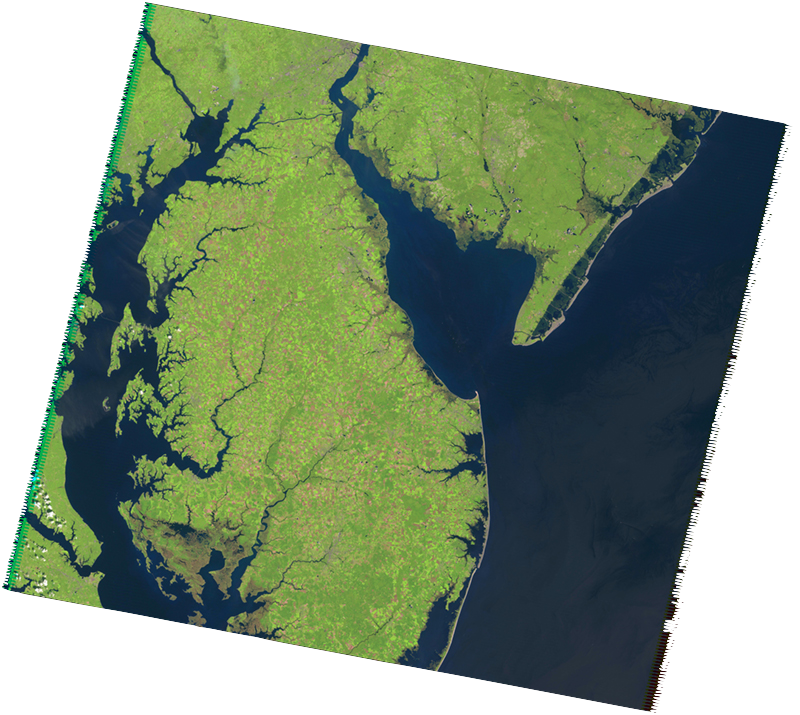
\includegraphics[scale=0.2]{landsat.png}
	\caption{An example of how a Landsat scene looks like.}
	\label{figurelabel}
\end{figure}

\section{Convolutional Neural Networks}

 Y with Z channels is equivalent to X $\times$ Y $\times$ Z single vector, which means that there needs to be X $\times$ Y $\times$ Z weights computed in the first hidden layer. And with additional hidden layers in the model, these number of weights scale up quickly. In addition, spatial context between pixels are not explicitly conserved in multilayer perceptrons. This is due to the flattening of dimensionality down to a single vector. As a result, each pixel is considered independently without considering the spatial locality in the image. Convolutional neural networks (CNNs) are a special type of multilayer neural networks that are inspired by the animal’s visual cortex. They can handle images as multidimensional input instead of single vectors and thus, spatial context of pixels is conserved. CNN architectures contain several unique features that make them the number one choice for image recognition and classification amongst other multilayer neural networks. These features include local connectivity of neurons, parameter sharing, pooling/subsampling and depth.

CNNs contain an important feature known as local connectivity. What this means is that neurons in a hidden layer are only connected to a sub region known as a receptive field of the input. This is different than multilayer perceptrons in which all the neurons are connected to all the neurons in the previous layer. Because of this, there is a lot fewer parameters required and as a result, the computation needed is a lot less. In addition, the structure of neurons in the hidden layer is dependence of the number of channels in the receptive field. With this fact that the number of channels is increasing after subsequent layers, having more layers can model long range dependencies more efficiently.

Another important feature of CNNs is parameter sharing. With parameter sharing, all the neurons belonging to a particular future map share the same weighted connections. These neurons, in addition, cover all the used perceptive fields. These weighted connections are also known as filters or kernels. Due to the fact that parameters shared by all neurons belong to a feature map, this also reduces the number of parameters by a lot. If using a specific filter, the feature map will extract the same feature at all the receptive fields. The combination of different feature maps builds multidimensional matrices, which in return generate the input for the next layer.

Another prominent feature of CNNs is pooling (or subsampling). Pooling is a layer that preforms two operations. On non-overlapping patches in the feature map, a pool of neighboring neurons is replaced by a single neuron. In subsampling, the pool generated neurons replace the pool of neighboring neurons in the next hidden layer. As a result, the dimensionality can drastically be reduced between convolution layers. There can be various different types of pools, such as maximum, minimum and average pool.
Lastly, depth, or the number of layers, is essential in CNNs. In general, we do not theoretically understand the advantages of having a deep architecture over shallow ones, however, they have shown to solve complex AI tasks such as image analysis and natural language processing. As a result, different experiments have shown that the growth that the number of neurons grows linearly in deep networks, while in the case of shallow networks they grow exponentially when representing the same functions. As a result, the architecture used in this research also uses the same idea in that the accuracy increases even if a single convolutional layer is removed.

These features, in combination, allow CNNs to be the favored architecture for image recognition and classification. These features allow for the model to learn complex relationships in the input data in an efficient manner, while extracting features and along through subsequent layers. In comparison to multilayer perceptrons, they require a lot less parameters and as a result are a lot more effective in learning multidimensional input data.

\section{Patch-based CNN for remote sensing image classification}


The patch-based CNN architecture that will be used for this research is tailored for medium-resolution remote sensing imagery however, it is also generic, and the model will work for any medium-resolution multidimensional data. This section focuses on highlighting the unique features of this architecture and the procedure used for preprocessing the data. This section will describe obtaining/calculating the multidimensional data, extracting various patches, cloud/shadow masking, selection of training samples, selection of hyperparameters and the model’s architecture.

\subsection{Preprocessing}

When obtaining the multidimensional Landsat 8 data, there is a series of preprocessing that must be done in order to get the data in the appropriate format to be processed as input to the CNN. Firstly, because the dataset is of medium-resolution and the spatial resolution is 30 m, we must overcome the limitation of not having fine structure in our data for use of the CNN to classify. One of these methods includes calculating top-of-atmosphere (TOA) reflectance value for each pixel in the input data. Originally, the data that is inputted is in the form of Digital Numbers. This value belongs to all the OLI bands except the panchromatic band. Digital Numbers is the measure of initial energy received at the input of the sensors on the satellite. However, due to atmospheric conditions and radiation from other mediums of light, calculating the TOA can essentially clean up the noise that is present from the atmosphere. To calculate these values, the Digital Numbers, which are represented in 16-bit unsigned integers, can be rescaled using radiometric reflectance coefficients and sun angle provided in the metadata file present in the dataset. As a result, a Landsat image is converted into multidimensional TOA reflectance matrix of size X $\times$ Y $\times$ Z where X is the width, Y is the height, and Z is the number of channels. For the Landsat images, TOA reflectance values are calculated for every pixel in the eight OLI bands. As a result, the matrix we obtain is of size X $\times$ Y $\times$ 8 where the 8 channels are represented by the 8 different OLI bands. The values of X $\times$ Y $\times$ Z vary with different medium-resolution image source; however, they are generic for any multidimensional data.

   \begin{figure}[thpb]
	\centering
	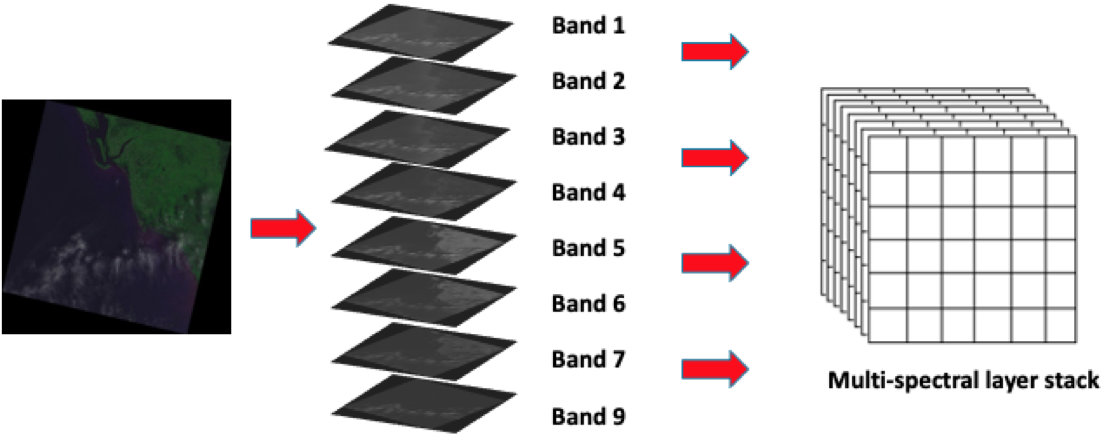
\includegraphics[scale=0.43]{preprocessing.png}
	\caption{How the bands are structured in the input data.}
	\label{figurelabel}
\end{figure}


As mentioned before, CNNs allow for multidimensional input instead of single vectors. Therefore, multidimensional samples must be extracted instead of pixel-based single vectors. Initially, patches of size 5 $\times$ 5 $\times$ 8 are extracted from the Landsat TOA matrix and labeled using the center pixel of the patch. The impact of using various patch sizes extracted from the TOA matrix has a significant impact on the accuracy and performance of the model. Patches of size 5 $\times$ 5 $\times$ 8 are initially extracted because they capture spatially local information with correlation of the center pixel and the surrounding pixels and limit the heterogeneous pixels. This size, however, may or may not be optimal. In addition, different classes may perform better on smaller patch sizes, while others perform better on larger patch sizes. As part of the experimentation of this research, different patch sizes are extracted and analyzed to observe the behavior of the model performance. As a result, patches of size 3 $\times$ 3 $\times$ 8, 7 $\times$ 7 $\times$ 8, 9 $\times$ 9 $\times$ 8, and 11 $\times$ 11 $\times$ 8 are also extracted. These patches are extracted for all possible locations in the data and patches overlap with neighboring patches. In order to extract the maximum number of samples from the dataset, a stride value of one is used for all the valid locations. The valid locations include anywhere within the boundary of the dataset, and anywhere where there are no clouds and shadows.

Inside the Landsat image, there are pixels that belong to clouds and shadows. To deal with this, a mask is generated to remove these pixels. The mask is produced using the FMask Algorithm. This algorithm scans the Landsat image and creates a mask of values of 1s and 0s. Values of 0s belong to cloud and shadows while values of 1s belong to anything else. This mask overlays the TOA reflectance matrix and as a result, any areas with clouds and shadows have a TOA value of zero. If patches contained any clouds and/or shadows, they are not used.

For selecting samples to be a part of the training set, two constraints are placed on the patches. The first constraint is that 60\% or more of the pixels present in a patch should belong to the same class as the center pixel. The next constraint is that there should be no cloud/shadow pixels present in the patch. If a patch satisfies these constraints, then it is extracted and used to be a part of the training set. This concludes the preprocessing needed for the dataset.


\subsection{The architecture}
The proposed CNN contains five convolution layers, a fully connected layer and a softmax layer. The structure can be seen in Fig. 3. All convolutions have a stride value of one and are zero padded. This is because the size of input sample is relatively small to begin with. If there were no padding used, the dimensionality of the patch would reduce quickly and thus a deep model could not be used. As a result, we add zero padding to keep the dimensionality of X $\times$ Y to be the same after convolution layers. The number of filters increases in powers of two beginning with 8 filters in the first convolution layer and ending with 64 in the fifth. This increases the number of feature maps in the hidden layers. For best results, five convolutional layers were discovered to be the optimal number of layers to use. Adding more layers did not improve accuracy and reducing layers decreased accuracy.

There were no pooling/subsampling layers used in the architecture because of the low dimensionality of input shape. The final softmax layer generates a probability distribution over the eight classes and it uses the output from the previous fully connected layer as input. The architecture was implemented in Keras and the backend used was Google's Tensorflow. In addition, a NVIDIA Quadro GP100 GPU was used for training. The loss function used is categorical cross entropy and this value is minimized using the ADAM optimizer using a learning rate of 0.0001. The ADAM optimizer is a first-order gradient-based optimization algorithm that incorporates features such as momentum. It is a very effective and popular optimization algorithm hence why it was used for this project. In addition, on every layer except the last layer, the activation function rectified linear unit (ReLU) is applied on the outputs generated from the neurons. The number of filters are doubling in subsequent convolution layers, the last fully connected layer has 3200 neurons.


   \begin{figure}[thpb]
	\centering
	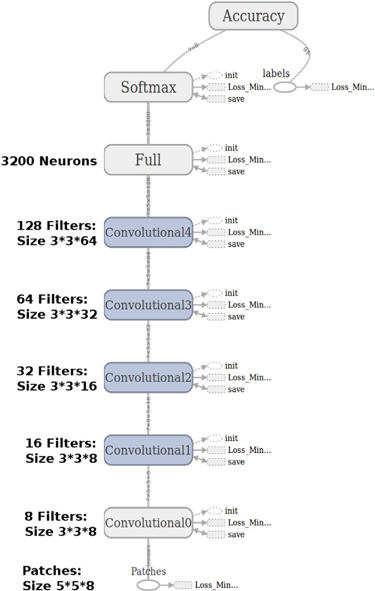
\includegraphics[scale=0.79]{arc.png}
	\caption{Architecture of the proposed convolutional neural network system.}
	\label{figurelabel}
\end{figure}


\section{Experimental results and comparisons}

Using the reference map as ground truth, the accuracy of the model is computed as the percentage of pixels outputted from the CNN that have the same label as the reference map. After 9999, 49999, 89999, 129999 and 149999 iterations, the architecture achieved 72.93\%, 79.12\%, 83.06\%, 84.67\% and 85.60\% validation accuracy respectively for patch size of 5 $\times$ 5 $\times$ 8.

The test site used was the Florida Everglades. The reason why this area is selected as the test site is because it contains a wide variety of sub-ecosystems such as tropical hardwood hammocks, freshwater marshes, mangrove swamps and cypress swamps. This kind of diverse ecosystem is a good site to use for testing as we can use it to analyze the robustness of the architecture. The image used from the Landsat 8 database was taken on February 10, 2014 with Path 16 Row 42. Only a certain subset of this image, however, is used for the test site. The size of the test site is 771 square kilometers with each pixel having a 30 m $\times$ 30 m spatial resolution. This makes the overall image have dimensionality of 864 $\times$ 991 pixels.

To create the reference map for the test site, ancillary data from the Florida Cooperative Land Cover Map was obtained. This data was then corrected by comparing it to high-resolution images obtained from Google Earth and with GPS-guided field observations. This reference map is then used to generate training samples in which accuracy assessments can then be performed. Using eight different classes, high intensity urban, low intensity urban, barren land, forest, cropland, woody wetland, emergent herbaceous wetland and water, patches of size 5 $\times$ 5 $\times$ 8 are initially extracted.

By comparing the performance of this model in comparison to the four different networks, pixel-based neural network achieves 62.34\% accuracy, pixel-based convolutional neural network achieves 63.01\% accuracy, patch-based neural network achieves 73.17\% accuracy and the patched based CNN used for this research achieves 85.60\% accuracy. In addition, accuracies of support vector machines and random forests are calculated and obtained as 61.86\% and 75.22\%. It is clear that the architecture used in this paper beats other previous forms of classification on medium resolution. In order to properly test the classification results, accuracy assessment using error matrix is performed. This error matrix uses the weighted random stratified sampling, and an overall accuracy is obtained based on the error matrix. The overall accuracy obtained achieves 89.26\% accuracy when patches of size 5 $\times$ 5 $\times$ 8 are used. In most classes, there is a significant improvement in accuracy in comparison to the other four different networks.

In comparison to single pixel-based neural network and CNN, the input is no longer a patch and therefore the vector is simply of length 8 of TOA reflectance values and 8 OLI bands. Both pixel-based neural network and CNN achieve almost similar results, so there is no improvement of using CNN over neural networks for single pixel-based input. It is clear that using patch-based input makes a significant impact on the classification accuracy. With this being said, if we can find the optimal patch size to use, then accuracy could potentially improve.

The motivation to explore different patch sizes and their behavior on the architecture is initially because of intuition leading to believe that some classes perform better on various patch sizes. This is because some areas, like high intensity urban, contain the same spatially local information. This means that most pixels that are labeled urban are all very near each other. When extracting a patch from an urban area, most of the pixels in that patch naturally belong to the same label as the center pixel. With this being said, there may not be a need to use a large patch size in order to accurately classify urban areas. On the other hand, some classes like emergent herbaceous wetland and woody wetland did not achieve as good of an accuracy as high intensity urban. This may be because there was not enough spatial information available within the patch to allow the pixel to be classified correctly. For cases like this, a larger patch size may perform better at classifying these classes. In theory, if dynamic sized patches were to be passed into the network with optimal sizes per class, the architecture would achieve better accuracy.

\begin{figure}[!b]
	\centering
	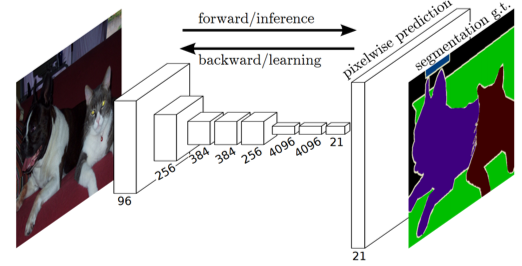
\includegraphics[scale=0.9]{fcn.png}
	\setlength{\belowcaptionskip}{-20pt}
	\caption{An example of a Fully Convolutional Network (FCN) for semantic segmentation.}
	\label{figurelabel}
\end{figure}

Patches of size 3 $\times$ 3 $\times$ 8, 7 $\times$ 7 $\times$ 8, 9 $\times$ 9 $\times$ 8, and 11 $\times$ 11 $\times$ 8 were also extracted. To train a network on various patch sizes is not an easy task. This is because convolutional neural networks typically depend input to be of fixed size. If we were to pass various size patches into the CNN, the architecture would not accept it because the fully connected layer at the end of the CNN determines the amount of weights it has based on the output dimension of the convolution layers. Because the shapes of the inputs are dynamic, so is the outputs of the convolutions, therefore the fully connected layer cannot construct the right amount of weights needed. To overcome this limitation, there are multiple approaches that can be taken. The first idea was to remove the fully connected layer. These types of architectures are known as Fully Convolutional Networks (FCN) and they are typically used for semantic segmentation. FCNs allow for variable sized input as they do not contain a fully connected layer. The output dimension would be the same as the input dimension and the model gives a pixel wise classification for every up sampled image from the network. Although using this architecture, at first, sounded like a good idea to implement, after further analysis it appeared that semantic segmentation is fundamentally solving a different problem and we could not use it for our case. This is because we’re using the spatial information within a patch to classify the center label, and not giving a pixel wise prediction of the patches. In addition, typically in FCNs, smaller patches are not passed in and instead the entire image is passed in as input. This means if we wanted to use FCNs, we would most likely be passing in the entire satellite image of our test site and we would not achieve good accuracy because of the large dimensionality and lack of spatial information. 

The next idea to allow variable sized input was by creating a form of ensemble network. This type of network would take the output of multiple other sub networks in order to give a final classification prediction. The sub networks would consist of individually trained networks that have fixed size input of the various patch sizes. To train these fixed sized networks on the patches individually was fortunately not a complicated procedure. The architecture did not have to be modified and the only hyperparameter changed was the input shape. Changing the input shape to be the same dimensionality of the patch size, the model was able to train individually on its own patch size. As a result, we had 5 different neural networks each trained on 3 $\times$ 3 $\times$ 8, 5 $\times$ 5 $\times$ 8, 7 $\times$ 7 $\times$ 8, 9 $\times$ 9 $\times$ 8, and 11 $\times$ 11 $\times$ 8 respectfully. The results of the network were surprising, however.

As the patch size increased, so did the validation accuracy. 3 $\times$ 3 $\times$ 8 achieved 79\% accuracy, 5 $\times$ 5 $\times$ 8 achieved 89\% accuracy, 7 $\times$ 7 $\times$ 8 achieved 93\% accuracy, 9 $\times$ 9 $\times$ 8 achieved 96\% accuracy, and 11 $\times$ 11 $\times$ 8 achieved 98\% accuracy. To understand why the accuracy has increased, we must look into the patches itself. After analyzing the datasets trained on, it appeared that the increase in accuracy was due to the fact of larger patch sizes being more homogeneous. This means that as patch size increased, the pixels in the patch were all mostly being the same label as the center pixel. This, in turn, makes it so that the data is bias and hence why the architecture achieved good validation accuracy. If these patches were put to the test, however, they would not achieve good accuracy because of the fact that they would not be able to classify areas that are not entirely homogeneous. This is why a patch size of 5 $\times$ 5 $\times$ 8 was used; because it limits the amount of heterogeneous pixels while still being able to generalize well.

To test if this is the case, the code was modified to extract patches of size 11 $\times$ 11 $\times$ 8 in areas where there were 60\% or more classes in areas of 3 $\times$ 3 $\times$ 8. This means that the patches were not as homogeneous. As a result, the accuracy of the 11 $\times$ 11 $\times$ 8 dropped to about 71\%. In order to effectively create a dataset that can be used for variable sized patches, we need to limit the number of homogeneous pixels within the patch as we increase the patch size. With this being said, in order to create an accurate form of weighted ensemble, more work needs to be done in producing an accurate training set.

\begin{figure}[htb]
	\centering
	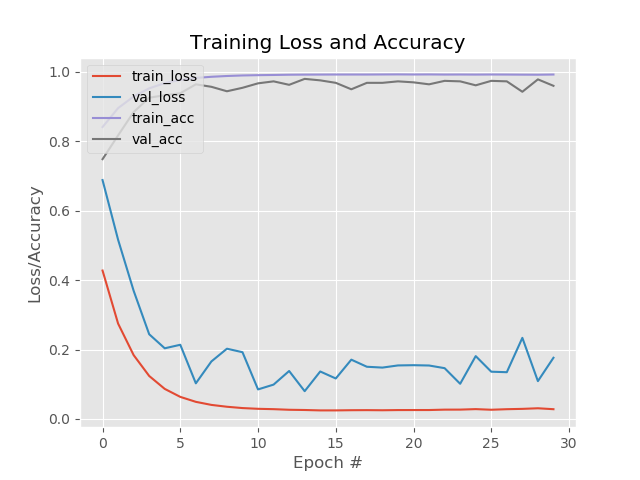
\includegraphics[scale=0.6]{results_9dim.png}
	\caption{Loss and accuracy plot for training 9 $\times$ 9 $\times$ 8 patch.}
	\label{figurelabel}
\end{figure}

\begin{figure}[htb]
	\centering
	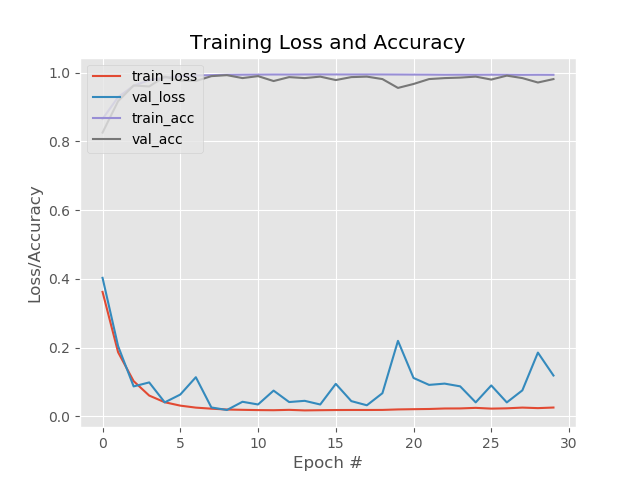
\includegraphics[scale=0.6]{results_11dim.png}
	\caption{Loss and accuracy plot for training 11 $\times$ 11 $\times$ 8 patch.}
	\label{figurelabel}
\end{figure}


\begin{figure*}[!t]
	\centering
	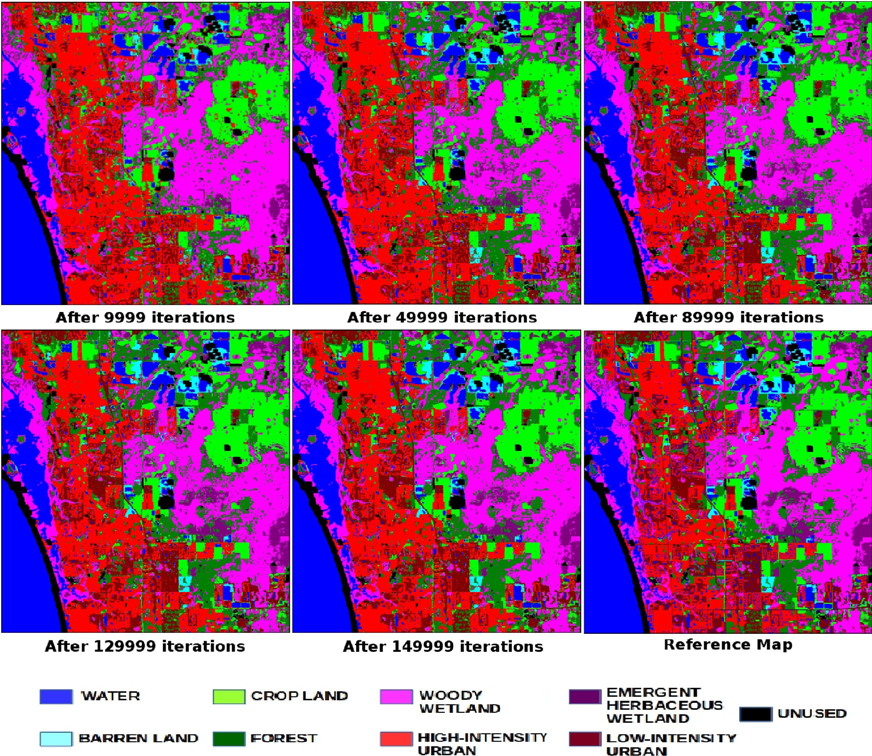
\includegraphics[scale=0.8]{iterations.png}
	\caption{Illustration of improvement in classification results with number of iterations. Compared to reference map, after certain number of iterations, the accuracy is as follows: (a) 9999 iterations: 72.93\%, (c) 49,999 iterations: 79.12\%, (d) 89,999 iterations: 83.06\%, (e) 129,999 iterations: 84.67\%, (f) 149,999 iterations: 85.60\%.}
	\label{figurelabel}
\end{figure*}

\begin{figure*}[!t]
	\centering
	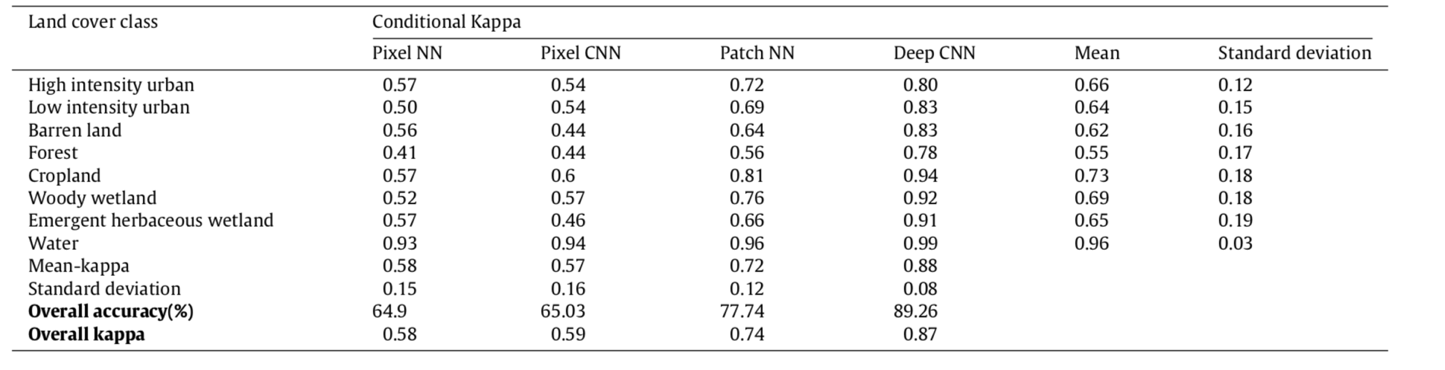
\includegraphics[scale=0.8]{comparisons.png}
	\caption{Summary of the accuracy assessment for the classification results produced by the new deep patch-based CNN system (Deep CNN), pixel-based neural network system (Pixel NN), pixel-based CNN (Pixel CNN) and multidimensional patch-based network system (Patch NN).}
	\label{figurelabel}
\end{figure*}




\section{CONCLUSION}

In this project, a patch-based CNN system for medium resolution remote sensing imagery classification was implemented and analyzed. This architecture uses multidimensional TOA reflectance values obtained from Landsat 8 satellite and patch-based samples were extracted and used for training. These patches contain spatial information and as a result the classification results achieve significant improvements in overall accuracies in comparison to the pixel-based conventional neural network, the pixel-based CNN and the patch-based neural network.

There are more changes and work to be done to increase the accuracy. We have analyzed different patch sizes and we have observed the behavior of using larger patch sizes on the architecture. To increase the accuracy of the model, a hierarchical structure classification using the same architecture can be built that works on different sizes patches for the same centered pixel. A weighted ensemble can then learn the optimal patch size for each class and create a gate to pass the input through the correct sized network for classification.

To apply this CNN system on the global level, convolution operations can be improved by incrementally updating the convolutions. This would make the computation more efficient. In addition, this architecture outputs a probability distribution over 8 classes. Textual constrains can be imposed on the class labels to improve the boundary accuracy. With this network, and with future work that can be added to the architecture, this proposed system can lead to more accurate global maps.




%\addtolength{\textheight}{-12cm}   % This command serves to balance the column lengths
                                  % on the last page of the document manually. It shortens
                                  % the textheight of the last page by a suitable amount.
                                  % This command does not take effect until the next page
                                  % so it should come on the page before the last. Make
                                  % sure that you do not shorten the textheight too much.

%%%%%%%%%%%%%%%%%%%%%%%%%%%%%%%%%%%%%%%%%%%%%%%%%%%%%%%%%%%%%%%%%%%%%%%%%%%%%%%%



%%%%%%%%%%%%%%%%%%%%%%%%%%%%%%%%%%%%%%%%%%%%%%%%%%%%%%%%%%%%%%%%%%%%%%%%%%%%%%%%



%%%%%%%%%%%%%%%%%%%%%%%%%%%%%%%%%%%%%%%%%%%%%%%%%%%%%%%%%%%%%%%%%%%%%%%%%%%%%%%%

%%%%%%%%%%%%%%%%%%%%%%%%%%%%%%%%%%%%%%%%%%%%%%%%%%%%%%%%%%%%%%%%%%%%%%%%%%%%%%%%

\begin{thebibliography}{99}

\bibitem{c1}Sharma, Atharva, Liu, Xiuwen, Yang, Xiaojun, Shi, Di. (2017). A patch-based convolutional neural network for remote sensing image classification. Neural Networks. 95. 10.1016/j.neunet.2017.07.017. 
\bibitem{c2}Abadi, Martín, Agarwal, Ashish, Barham, Paul, Brevdo, Eugene, Chen, Zhifeng, \& Citro, Craig et al. (2015). TensorFlow: Large Scale Machine Learning on Heterogeneous Systems. Software available from tensorflow.org.
\bibitem{c3}Anderson, James Richard (1976). A land use and land cover classification system for use with remote sensor data, Vol. 964. US Government Printing Office.
\bibitem{c4}Bartholome, E., \& Belward, A. S. (2005). Glc2000: a new approach to global land cover mapping from earth observation data. International Journal of Remote Sensing, 26(9).
\bibitem{c5}Bengio, Yoshua (2009). Learning deep architectures for AI. Foundations and Trends in Machine Learning, 2(1), 1–127.
\bibitem{c6}Bengio, Yoshua, LeCun, Yann, et al. (2007). Scaling learning algorithms towards AI. Large Scale Kernel Machines, 34(5).
\bibitem{c7}Berberoglu, S., Lloyd, Christopher D., Atkinson, P. M., \& Curran, Paul J. (2000). The integration of spectral and textural information using neural networks for land cover mapping in the Mediterranean. Computers \& Geosciences, 26(4), 385–396.
\bibitem{c8}Blaschke, Thomas (2010). Object based image analysis for remote sensing, International Journal of Photogrammetry and Remote Sensing, 65(01).
\bibitem{c9}Blaschke, Thomas, Hay, Geoffrey J., Kelly, Maggi, Lang, Stefan, Hofmann, Peter, Addink, Elisabeth, et al. (2014). Geographic object based image analysis towards a new paradigm. International Journal of Photogrammetry and Remote Sensing, 87(0).
\bibitem{c10}Boureau, Y-Lan, Ponce, Jean, \& LeCun, Yann (2010). A theoretical analysis of feature pooling in visual recognition. In Proceedings of the 27th international conference on machine learning, ICML 10 (pp. 111–118).
\bibitem{c11}Castelluccio, Marco, Poggi, Giovanni, Sansone, Carlo, \& Verdoliva, Luisa (2015). Land use classification in remote sensing images by convolutional neural networks, ArXiv Preprint arXiv:1508.00092.
\bibitem{c12}Collobert, Ronan, \& Weston, Jason (2008). A unified architecture for natural language processing: Deep neural networks with multitask learning. In Proceedings of the 25th international conference on machine learning (pp. 160–167). ACM.
\bibitem{c13}Congalton, Russell G. (1991). A review of assessing the accuracy of classifications of remotely sensed data. Remote Sensing of Environment, 37(1), 35–46.
\bibitem{c14}Davis, Steve, \& Ogden, John C. (1994). Everglades: the ecosystem and its restoration. CRC Press.
\bibitem{c15}Delalleau, Olivier, \& Bengio, Yoshua (2011). Shallow vs. deep sumproduct networks. In Advances in neural information processing systems (pp. 666–674). Deng, Li, Li, Jinyu, Huang, Jui-Ting, Yao, Kaisheng, Yu, Dong, Seide, Frank, et al.
\bibitem{c16}(2013). Recent advances in deep learning for speech research at Microsoft. In 2013 IEEE international conference on acoustics, speech and signal processing (pp. 8604–8608). IEEE.
\bibitem{c17}Foley, Jonathan A., DeFries, Ruth, Asner, Gregory P., Barford, Carol, Bonan, Gordon, Carpenter, Stephen R., et al. (2005). Global consequences of land use. Science, 309(5734).
\bibitem{c18}Fry, J. A., Xian, G., Jin, S., Dewitz, J. A., Homer, C. G., Yang, L., et al. (2011). Completion of the 2006 national land cover database for the conterminous united states. Photogrammetric Engineering and Remote Sensing, 77.
\bibitem{c19}Fukushima, Kunihiko, \& Miyake, Sei (1982). Neocognitron: A self organizing neural network model for a mechanism of visual pattern recognition. In Competition and cooperation in neural nets (pp. 267–285). Springer.
\bibitem{c20}Gidudu, Anthony, Hulley, Greg, \& Marwala, Tshilidzi (2007). Classification of images using support vector machines, CoRR ( arXiv:0709-3967v1).
\bibitem{c21}Gong, Peng, Wang, Jie, Yu, Le, Zhao, Yongchao, Zhao, Yuanyuan, Liang, Lu, et al. (2013). Finer resolution observation and monitoring of global land cover: first mapping results with landsat tm and etm+ data. International Journal of Remote Sensing, 34(7).
\bibitem{c22}He, Kaiming, Zhang, Xiangyu, Ren, Shaoqing, \& Sun, Jian (2015). Deep Residual Learning for Image Recognition, ArXiv Preprint arXiv:1512.03385.
\bibitem{c23}Hinton, Geoffrey, Deng, Li, Yu, Dong, Dahl, George E, Mohamed, Abdel rahman, Jaitly, Navdeep, et al. (2012). Deep neural networks for acoustic modeling in speech recognition: The shared views of four research groups. IEEE Signal Processing Magazine, 29(6), 82–97.
\bibitem{c24}Hinton, Geoffrey E., \& Salakhutdinov, Ruslan R. (2006). Reducing the dimensionality of data with neural networks. Science, 313(5786), 504–507.
\bibitem{c25}Homer, C., Dewitz, J., Fry, J., Coan, M., Hossain, N., Larson, C., et al. (2001). Completion of the 2001 national land cover database for the conterminous united states. Photogrammetric Engineering and Remote Sensing, 73.
\bibitem{c26}Hu, Wei, Huang, Yangyu, Wei, Li, Zhang, Fan, \& Li, Hengchao (2015). Deep convolutional neural networks for hyperspectral image classification. Journal of Sensors, 2015.
\bibitem{c27}Huang, Kal-Y. I. (2002). A synergistic automatic clustering technique (SYNERACT) for multispectral image analysis. Photogrammetric Engineering and Remote Sensing, 68(1).
\bibitem{c28}Hubel, David H., \& Wiesel, Torsten N. (1968). Receptive fields and functional architecture of monkey striate cortex. The Journal of Physiology, 195(1), 215–243. Jensen, John R. (2015). Introductory digital image processing: a remote sensing perspective. (4th ed.). Pearson Education, Inc..
\bibitem{c29}Jin, Suming, Yang, Limin, Danielson, Patrick, Homer, Collin, Fry, Joyce, \& Xian, George
\bibitem{c30}(2013). A comprehensive change detection method for updating the national land cover database to circa 2011. Remote Sensing of Environment, 132(0). Kanellopoulos, I., \& Wilkinson, G. G. (1997). Strategies and best practice for neural network image classification. International Journal of Remote Sensing, 18(4), 711–725.
\bibitem{c31}Kavzoglu, T., \& Mather, P. M. (2003). The use of backpropagating artificial neural networks in land cover classification. International Journal of Remote Sensing, 24(23).
\bibitem{c32}Kingma, Diederik, \& Ba, Jimmy (2014). Adam: A method for stochastic optimization, ArXiv Preprint arXiv:1412.6980.
\bibitem{c33}Krizhevsky, Alex, Sutskever, Ilya, \& Hinton, Geoffrey E. (2012). Imagenet classification with deep convolutional neural networks. In Advances in neural information processing systems, Vol. 25. Curran Associates, Inc..
\bibitem{c34}Lillesand, Thomas M., Kiefer, Ralph W., \& Chipman, Jonathan W. (2008). Remote sensing and image interpretation. (6th ed.). John Wiley and Sons, Inc..
\bibitem{c35}Lloyd, Christopher D., Berberoglu, S., Curran, Paul J., \& Atkinson, Peter M. (2004). A comparison of texture measures for the perfield classification of Mediterranean land cover. International Journal of Remote Sensing, 25(19), 3943–3965.
\bibitem{c36}Lo, C. P., \& Watson, Lee J. (1998). The influence of geographic sampling methods on vegetation map accuracy evaluation in a swampy environment. Photogrammetric Engineering and Remote Sensing, 64(12), 1189–1200.
\bibitem{c37}Long, J., Shelhamer, E., and Darrell, T. Fully convolutional networks for semantic segmentation. CoRR,
abs/1411.4038, 2014
\bibitem{c38}Mas, J. F., \& Flores, J. J. (2008). The application of artificial neural networks to the analysis of remotely sensed data. International Journal of Remote Sensing, 29(3). Meyer, William B., \& Turner II, B. L. (1994). Changes in land use and land cover: a global perspective, Vol. 4. Cambridge University Press.
\bibitem{c39}Mountrakis, Giorgos, Im, Jungho, \& Ogole, Caesar (2011). Support vector machines in remote sensing: A review. International Journal of Photogrammetry and Remote Sensing, 66.
\bibitem{c40}Nair, Vinod, \& Hinton, Geoffrey E. (2010). Rectified linear units improve restricted boltzmann machines. In Proceedings of the 27th international conference on machine learning, ICML-10 (pp. 807–814).
\bibitem{c41}Nogueira, Keiller, Penatti, Otávio A. B., \& Dos Santos, Jefersson A. (2016). Towards Better Exploiting Convolutional Neural Networks for Remote Sensing Scene Classification, ArXiv Preprint arXiv:1602.01517.
\bibitem{c42}Pal, M. (2005). Random forest classifier for remote sensing classification. International Journal of Remote Sensing, 26(1).
\bibitem{c43}Pal, M., \& Mather, P. M. (2005). Support vector machines for classification in remote sensing. International Journal of Remote Sensing, 26(5), 1007–1011.
\bibitem{c44}Penatti, Otávio A. B., Nogueira, Keiller, \& dos Santos, Jefersson A. (2015). Do deep features generalize from everyday objects to remote sensing and aerial scenes domains? In Proceedings of the IEEE conference on computer vision and pattern recognition workshops (pp. 44–51).
\bibitem{c45}Romero, Adriana, Gatta, Carlo, \& Camps Valls, Gustau (2016). Unsupervised deep feature extraction for remote sensing image classification. IEEE Transactions on Geoscience and Remote Sensing, 54(3), 1349–1362.
\bibitem{c46}Russakovsky, Olga, Deng, Jia, Su, Hao, Krause, Jonathan, Satheesh, Sanjeev, Ma, Sean, et al. (2015). Imagenet large scale visual recognition challenge. International Journal of Computer Vision, 115(3), 211–252.
\bibitem{c47}Sermanet, Pierre, Eigen, David, Zhang, Xiang, Mathieu, Michaël, Fergus, Rob, \& LeCun, Yann (2013). Overfeat: Integrated recognition, localization and detection using convolutional networks, ArXiv Preprint arXiv:1312.6229.
\bibitem{c48}Shupe, Scott M., \& Marsh, Stuart E. (2004). Coverand densitybased vegetation classifications of the Sonoran Desert using Landsat TM and ERS-1 SAR imagery. Remote Sensing of Environment, 93(1), 131–149.
\bibitem{c49}Socher, Richard, Lin, Cliff C., Manning, Chris, \& Ng, Andrew Y. (2011). Parsing natural scenes and natural language with recursive neural networks. In Proceedings of the 28th international conference on machine learning, ICML-11 (pp. 129–136).
\bibitem{c50}Strahler, Alan H. (1980). The use of prior probabilities in maximum likelihood classification of remotely sensed data. Remote Sensing of Environment, 10(2).
\bibitem{c51}USGS. (2016a). Landsat Data Access, http://landsat.usgs.gov/Landsat\_Search\_and\_Download.php [Online; accessed 11.08.18].
\bibitem{c52}USGS. (2016b). Using the USGS Landsat 8 Product, http://landsat.usgs.gov/Landsat8\_Using\_Product.php [Online; accessed 11.08.18].
\bibitem{c53}Vogelmann, James E., Howard, Stephen M., Yang, Limin, Larson, Charles R., Wylie, Bruce K., \& Van Driel, Nicholas J. (2001). Completion of the 1990s national land cover data set for the conterminous united states from landsat thematic map per data and ancillary data sources. Photogrammetric Engineering and Remote Sensing, 67(6).
\bibitem{c54}Xu, Min, Watanachaturaporn, Pakorn, Varshney, Pramod K., \& Arora, Manoj K. (2005). Decision tree regression for soft classification of remote sensing data. Remote Sensing of Environment, 97(3).
\bibitem{c55}Yang, Xiaojun (2011). Use of Archival Landsat Imagery to Monitor Urban Spatial Growth. Urban Remote Sensing: Monitoring, Synthesis and Modeling in the Urban Environment, 15–33.
\bibitem{c56}Zhao, Wenzhi, \& Du, Shihong (2016). Spectral–spatial feature extraction for hyperspectral image classification: A dimension reduction and deep learning approach. IEEE Transactions on Geoscience and Remote Sensing, 54(8), 4544– 4554.
\bibitem{c57}Zhu, Zhe, \& Woodcock, Curtis E. (2012). Object based cloud and cloud shadow detection in Landsat imagery. Remote Sensing of Environment, 118.






\end{thebibliography}




\end{document}